\documentclass{beamer}
\usetheme{default}




\title{R vs. Python:}
\author{Katherine Encarnacion} 
\date{December 18, 2015}
\subtitle{for Data Analysis}
\institute{MATG 611}

\begin{document}


\begin{frame}
\titlepage
\end{frame}

\section{Introduction}


\subsection{Introduction}

\begin{frame}
\frametitle{Introcuction}
\begin{itemize}
\setlength\itemsep{3em}
\item Using Python to Reproduce midterm 2
\item What is Python?
\item What is R?
\item Data Manipulation
\end{itemize}
\end{frame}

\subsection{Python Packages and Libraries}


\begin{frame}
\frametitle{Python Packages and Libraries}
\begin{columns}
\column{0.5\textwidth}
\begin{itemize}
\setlength\itemsep{1em}
\item Importance of libraries and packages in Python
\item NumPy
\item Pandas
\item csv
\item matplotlib
\end{itemize}
\column{0.5\textwidth}
\begin{figure}
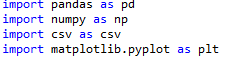
\includegraphics[width=2in]{import.png}
\caption{\label{Imported libraries and Packages}Imported libraries and Packages} 
\end{figure} 
\end{columns}
\end{frame}

\subsection{Problem 1}

\begin{frame}
\frametitle{Problem 1}
\begin{itemize}
\setlength\itemsep{3em}
\item Find the mean of the heart rate of each subject
\item Simple syntax
\item Errors within the book
\item Easier to learn then R
\end{itemize}
\end{frame}

\section{Result}
\subsection{Problem 1}

\begin{frame}
\frametitle{Problem 1 }
\begin{figure}
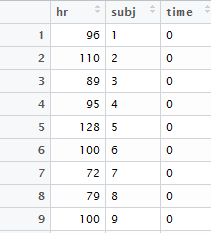
\includegraphics[scale=0.7]{heartratedata.png}
\caption{\label{fig:your-figure}Problem 1} 
\end{figure} 
\end{frame}


\subsection{Incorrect Syntax}

\begin{frame}
\frametitle{Incorrect Syntax}
\begin{figure}
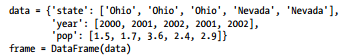
\includegraphics[scale=0.9]{dataframe.png}
\caption{\label{fig:your-figure}Python for Data Analysis Book} 
\end{figure} 
\end{frame}

\subsection{R results for problem 1}

\begin{frame}
\frametitle{R Results for Problem 1}
\begin{figure}
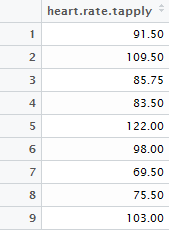
\includegraphics[scale=0.9]{displayP1R.png}
\caption{\label{fig:your-figure}Problem 1 Part a in R} 
\end{figure} 
\end{frame}

\subsection{Python results for problem 1}

\begin{frame}
\frametitle{Python Results for Problem 1}
\begin{figure}
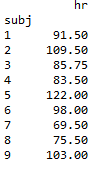
\includegraphics[scale=0.9]{displayP1Python.png}
\caption{\label{fig:your-figure}Problem 1 Part a in Python} 
\end{figure} 
\end{frame}



\subsection{Problem 2}

\begin{frame}
\frametitle{Problem 2}
\begin{itemize}
\setlength\itemsep{3em}
\item Creating factors 
\item Creating levels
\item Similar Syntax to R
\item Used counting function instead of creating a table
\end{itemize}
\end{frame}

\subsection{Python Syntax for problem 2}

\begin{frame}
\frametitle{Python Syntax for Problem 2}
\begin{figure}
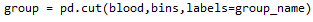
\includegraphics[scale=0.9]{PP2.png}
\caption{\label{fig:your-figure}Problem 2 in Python using Cut function} 
\end{figure} 
\end{frame}


\subsection{R Syntax for problem 2}

\begin{frame}
\frametitle{R Syntax for Problem 2}
\begin{figure}

\includegraphics[scale=0.6]{RP2.png}
\caption{\label{fig:your-figure}Problem 2 in R using the Cut function} 
\end{figure} 
\end{frame}


\subsection{Conclusion}

\begin{frame}
\frametitle{Conclusion}
\begin{itemize}
\setlength\itemsep{3em}
\item It is quite difficult to learn new syntax in 2 days.
\item Both are very similar.
\item Difficulty solving problem 3.
\item Prefer R for data analysis.
\end{itemize}
\end{frame}



\end{document}